
\label{sec:model} 
%We define here a hierarchically supervised LDA
%model. Although we will focus on document modeling in our description
%and experiments, this model applies equally well to other collections
%of discrete data with hierarchically constrained labels. 

HSLDA is a model for hierarchically, multiply-labeled, bag-of-words data.  We will refer to individual groups of bag-of-word data as documents.  Let $w_{n,d} \in \Sigma$ be the $n$th observation in the $d$th document.  Let $\mathbf{w}_d = \{w_{1,d},\ldots,w_{1,N_d}\}$ be the  set of $N_d$ observations in document $d$.  Let there be $D$ such documents and let the size of the vocabulary be $V=|\Sigma|$.  Let the set of labels be $\mathcal{L}=\left\{ l_{1},l_{2},\ldots,l_{\left|\mathcal{L}\right|}\right\} $. Each label except root labels $l \in \mathcal{L}$ has a parent $\mathrm{pa}(l) \in \mathcal{L}$ also in the set of labels.
 We will for exposition purposes assume that this label set has hard ``is-a'' parent-child constraints (explained later), although this assumption can be relaxed at the cost of more complicated inference.  Such a label hierarchy forms a multiply rooted tree.  Without loss of generality we will consider a tree with a single root $r\in\mathcal{L}$.  Each document has a variable $y_{l,d} \in \{-1,1\}$ for every label which indicates whether the label is applied to document $d$ or not.   In most cases $y_{i,d}$ will be unobserved, in some cases we will be able to fix its value because of  constraints on the label hierarchy, and in the relatively minor remainder its value will be observed.  In the applications we consider, only positive label applications are observed.  
 
The constraints imposed by an is-a label hierarchy are that if the $l$th label is applied to document $d$, i.e.~$y_{l,d} = 1$, then all labels in the label hierarchy up to the root are also applied to document $d$, i.e.~$y_{\mathrm{pa}(l),d} = 1, y_{\mathrm{pa}(\mathrm{pa}(l)),d} = 1, \ldots, y_{r,d}=1.$  Conversely, if a label $l'$ is marked as not applying to a document then no descendant of that label may be applied to the same.   We assume that at least one label is applied to every document.  This is illustrated in Figure~\ref{fig:graphical_model} where the root label is always applied but only some of the descendant labelings are observed as having been applied (diagonal hashing indicates that potentially some of the plated variables are observed).
%To reiterate, these is-a label hierarchy constraints can be relaxed.
%To capture this hierarchical structure we model the labeling of documents
%using a generative cascade of conditional probit regression models.

% generalize to arbitrary codes (not just ICD-9's
%
\begin{figure}[t]
%tbp] %  figure placement: here, top, bottom, or page
 \centering 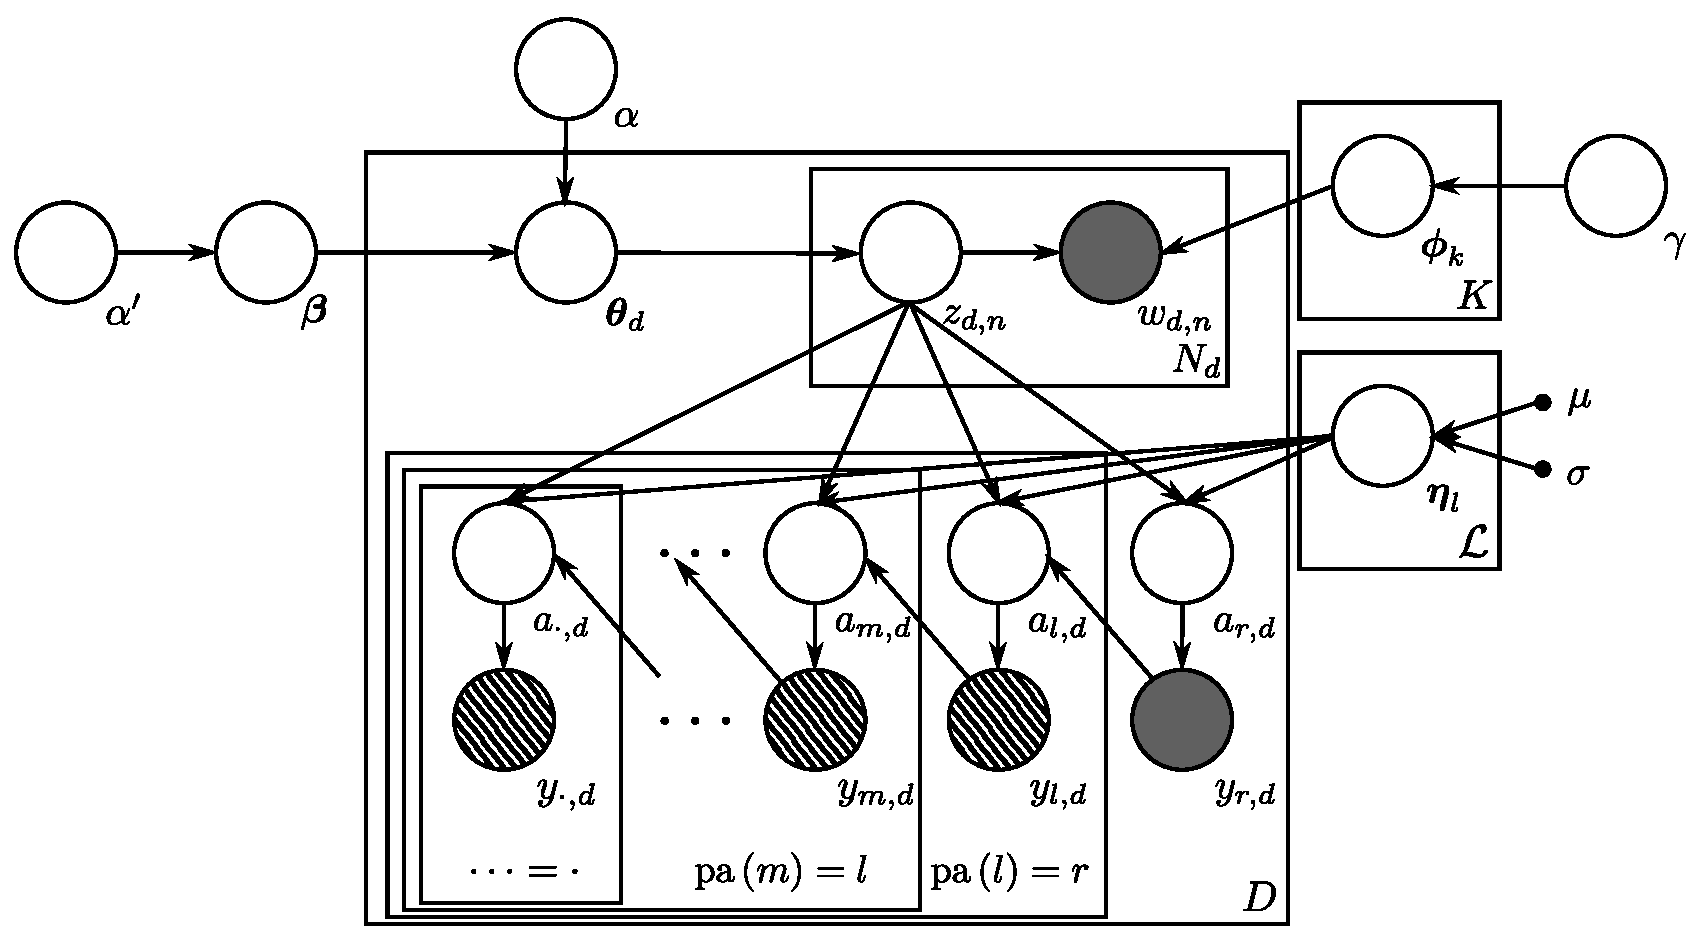
\includegraphics[scale=0.4]{Graphical_Model-final} \caption{HSLDA graphical model}


\label{fig:graphical_model} 
\end{figure}

In HSLDA, the bag-of-words document data is modeled using the LDA mixed-membership mixture model with global topic estimation.  Label responses are generated using a conditional hierarchy of probit regressors.   The HSLDA graphical model is given in Figure~\ref{fig:graphical_model}. In it and the following $K$ is the number of LDA "topics" (distributions over the elements of $\Sigma$), $\boldsymbol\phi_k$ is a distribution over ``words,'' $\boldsymbol\theta_d$ is a document-specific distribution over topics, $\boldsymbol\beta$ is a global distribution over topics, Dir$_{K}(\cdot)$ is a $K$-dimensional Dirichlet distribution, $\mathcal{N}_{K}(\cdot)$ is the $K$-dimensional Normal distribution, $\mathbf{I}_{K}$ is the $K$ dimensional identity matrix,  $\mathbf{1}_d$ is the $d$-dimensional vector of all ones, and $\mathbb{I}(\cdot)$ is an indicator function that takes the value $1$ if its argument is true and $0$ otherwise.  The following procedure describes how to generate from the HSLDA generative model.

 %as well as the mean, $\boldsymbol\mu$, and the standard deviation, $\sigma$,
%used in a normal prior distribution. The hyper-parameters $\alpha^{\prime}$,
%$\alpha$, and $\gamma$ are weight parameters for Dirichlet prior
%distributions. 


%We will now describe the stochastic generative process which defines
%our model. The 
%Given the number of topics, K, and broad gamma priors on hyperparameters,
%the generative process is as follows: 

\begin{enumerate}
\item For each topic $k=1,\ldots,K$

\begin{itemize}
\item Draw a distribution over words $\boldsymbol\phi_{k}\sim{\rm Dir}_{V}(\gamma\mathbf{1}_V)$%,
%where $\mathbf{1}$ is a vector of ones of length $V$ 
\end{itemize}
\item For each label $l\in\mathcal{L}$

\begin{itemize}
\item Draw a label application coefficient $\boldsymbol\eta_{l}\mid\mu,\sigma\sim\mathcal{N}_{K}(\mu \mathbf{1}_K,\sigma \mathbf{I}_{K})$  
\end{itemize}
\item Draw the global topic proportions $\boldsymbol\beta\mid\alpha'\sim{\rm Dir}_{K}\left(\alpha^{\prime}\mathbf{1}_K\right)$
\item For each document $d=1,\ldots,D$

\begin{itemize}
\item Draw topic proportions $\boldsymbol\theta_d\mid\boldsymbol\beta,\alpha\sim{\rm Dir}_{K}\left(\alpha\boldsymbol\beta\right)$ 
\item For $n=1,\ldots,N_{d}$

\begin{itemize}
\item Draw topic assignment $z_{n,d}\mid\boldsymbol\theta_d\sim{\rm Multinomial}(\boldsymbol\theta_d)$ 
\item Draw word $w_{n,d}\mid z_{n,d},\boldsymbol\phi_{1:K}\sim{\rm Multinomial}(\boldsymbol\phi_{z_{n,d}})$ 
\end{itemize}
\item Set $y_{r,d} = 1$
\item For each label $l$ in a breadth first traversal of $\mathcal{L}$ starting at the children of  root $r$

\begin{itemize}
\item Draw $a_{l,d}\mid \bar{\mathbf{z}}_d,\boldsymbol\eta_{l},y_{\mathrm{pa}(l),d}\sim\begin{cases}
\mathcal{N}(\bar{\mathbf{z}}^{T}_d\boldsymbol\eta_{l},1), & y_{\mathrm{pa}(l),d}=1\\
\mathcal{N}(\bar{\mathbf{z}}^{T}_d\boldsymbol\eta_{l},1)\mathbb{I}(a_{l,d}<0), & y_{\mathrm{pa}(l),d}=-1\end{cases}$ %\item Draw $a_{l, d} \ | \ z_{1:N_d,d}, \boldsymbol\beta_l \sim \mathcal{N} \left(\bar z_d^{T} \boldsymbol\beta_{l},1\right)$, where $\bar z_d=N_d^{-1}\sum_{n=1}^{N_d}z_{n,d}$ 
 
\item Apply label $l$ to document $d$ according to $a_{l,d}$ \[\hspace{-2cm}
y_{l,d}\mid a_{l,d}=\begin{cases}
\ \ \ 1 & \text{if \ensuremath{a_{l,d}>0}} \\% and \ensuremath{y_{{\rm \mathrm{pa}}(l),d}=1}}\\
-1 & \text{otherwise}\end{cases}\]
 
\end{itemize}
\end{itemize}
\end{enumerate}


Here $\bar{\mathbf{z}}_d^T = [\bar{z}_{1}, \ldots, \bar{z}_k, \ldots, \bar{z}_K]$ is the empirical topic distribution for document $d$, in which each entry is the percentage of the words in that document that come from topic $k$, $\bar{z}_{k}=N_{d}^{-1}\sum_{n=1}^{N_d}\mathbb{I}(z_{n,d}=k).$ 

The second half of step 4 is a substantial part of our contribution to the general class of supervised LDA models.  Here each document is generatively labeled using a hierarchy of conditionally dependent probit regressors \cite{gelman?,probit_regression?}.  For every label $l \in \mathcal{L}$ both the empirical topic distribution for document $d$ and whether or not its parent label was applied (i.e.~$\mathbb{I}(y_{\mathrm{pa}(l),d}=1)$) are used to decide whether or not  label $l$ is to be applied to  document $d$ as well.  Note that label $y_{l,d}$ can only be applied to document $d$ if its parent label $\mathrm{pa}(l)$ is also applied (these expressions are specific to is-a constraints but can be modified to accommodate different constraints).  The regression coefficients $\boldsymbol\eta_l$ are independent a priori, however, the hierarchical coupling in this model induces a posteriori dependence.   The net effect of this is that label predictors deeper in the label hierarchy are able to focus on finding specific, conditional labeling features.  We believe this to be a significant source of the empirical label prediction improvement we observe experimentally.  We test this hypothesis in Section~\ref{sec:experiments}.

Note that the choice of variables $a_{l,d}$ and how they are distributed were  driven at least in part by posterior inference efficiency considerations.  In particular, choosing probit-style auxiliary variable distributions for the $a_{l,d}$'s  yields conditional posterior distributions for both the auxiliary variables \eqref{eqn:a_l_d} and the regression coefficients \eqref{eqn:regression_param_conditional} which are analytic.  This simplifies posterior inference substantially.

%Probit regression is similar to logistic regression except that it uses the standard normal distribution cumulative distribution function (CDF) rather than the logistic sigmoid link function.  The inverse of the normal CDF is is known as the probit function.  
%The latent variables $a_{l,d}$ are
%auxiliary variables because the are introduced to make exact Gibbs
%sampling possible and are not of primary interest.

%This type of generative model is known as a probit regression model.
%Probit regression models are a type of discriminative probabilistic
%model similar to logistic regression. However, instead of using the
%logistic sigmoid as the link function, the probit regression model
%uses the CDF for a standard normal distribution - the inverse of which
%is known as the probit. In this case, the regression is conditional
%on the parents according to the constraints of the labeling hierarchy.

In the common case where no negative labels are observed (like the example applications we consider in Section~\ref{sec:experiments}), the model must be explicitly biased towards generating data that has negative labels in order to keep it from learning to assign all labels to all documents.   This is a common problem in modeling unbalanced data.  To see how this model can be biased in this way we draw the readers attention to the $\mu$ parameter and, to a lesser extent, the $\sigma$ parameter above.  Because $\bar{\mathbf{z}}_d$ is always positive, setting $\mu$ to a negative value results in a bias towards negative labelings, i.e.~for large negative values of $\mu$, all labels become a priori more likely to be negative ($y_{l,d}=-1$).  We explore the ability of $\mu$ to bias out-of-sample label prediction performance in Section~\ref{sec:experiments}.

%we apply an informative
%prior to the regression parameters, $\mathbf{\boldsymbol\beta}_{\mathcal{L}}$,
%in the form of a negative prior that encodes a bias towards being
%truly negative in the absence of a label.

